% !TEX root = rob1.tex
\chapter{Teilsysteme eines Roboters}

\section{Mechanische Komponenten}
\subsection{Gelenktyp}
\begin{compactitem}
    \item \textbf{Rotationsgelenk (R)}: Drehachse rechtwinkling zu beiden Achsen. Ellenbogengelenk
    \item \textbf{Torsionsgelenk (T)}: Drehachse parallel zu den Achsen beider Glieder. Unterarmdrehung
    \item \textbf{Revolvergelenk (V)}: Eingangsglied parallel zur Drehachse, Ausgangsglied rechtwinkling.
    Schultergelenk.
    \item \textbf{Lineargelenk (L)}: Gleitende oder fortschreitende Bewegung entlang der Achse.
    Translationsgelenk, Schubgelenk oder prismatisches Gelenk
\end{compactitem}
\subsection{Arbeitsraum}
Arbeitsraum besteht aus den Punkten im 3D Raum, die von der Roboterhand angefahren
werden können. Mindestens drei Bewegungsfreiheitsgrade erforderlich. \\
\textbf{Grundform} des Arbeitsraums, ist der Raum, der sich ergeben würde, wenn man die gegenseitige
Behinderung der Arme und die Begrenzungen der Gelenkwinkel nicht berücksichtigt.

\subsubsection{Räumliche Koordinatensysteme}
\begin{compactitem}
    \item \textbf{Kartesisch Koordinaten}: $P(x,y,z)$
    \item \textbf{Kugelkoordinaten}:$P(r,\alpha,\beta)$
    \item \textbf{Zylinderkoordinaten}: $P(r,\alpha,z)$
\end{compactitem}

\mparagraph{Umrechnung}
Kartesische Koordinaten $\rightarrow$ Kegelkoordinaten, $(x,y,z) \rightarrow (r,\alpha,z)$
\begin{align}
r &= \sqrt{x^2+y^2}\\
\alpha &= \arctan(\frac{y}{x})\\
z &= z
\end{align}

Kegelkoordinaten $\rightarrow$ Kartesische Koordinaten, $(r,\alpha,z) \rightarrow (x,y,z)$
\begin{align}
x &= r \cos(\alpha)\\
y &= r \sin(\alpha)\\
z &= z
\end{align}

Kartesische Koordinaten $\rightarrow$ Kugelkoordinaten, $(x,y,z) \rightarrow (r,\alpha,\beta)$
\begin{align}
    r &= \sqrt{x^2+y^2+z^2}\\
    \alpha &= \arctan{\frac{y}{x}}\\
    \beta &= \arctan{\frac{z}{\sqrt{x^2+y^2}}}
\end{align}

Kugelkoordinaten $\rightarrow$ Kartesische Koordinaten, $(r,\alpha,\beta) \rightarrow (x,y,z)$
\begin{align}
    x &= r \sin(\alpha)\cos(\beta)\\
    y &= r \sin(\alpha)\sin(\beta)\\
    z &= r \cos(\alpha)
\end{align}

\subsection{Radkonfigurationen}

\begin{table}[h!]
\centering
\begin{tabular}{|l|l|l|l|}
\hline
\textbf{Antrieb}             & \multicolumn{1}{c|}{\textbf{Eigenschaften}}                                                                                                   & \multicolumn{1}{c|}{\textbf{Vorteile}}                                                               & \multicolumn{1}{c|}{\textbf{Nachteile}}                                             \\ \hline
\textbf{Differentialantrieb} & \begin{tabular}[c]{@{}l@{}}- Geradeaus- und Kurvenfahrt\\ - Drehen auf der Stelle\\ - Vorwärts und Rückwärtsfahren \\ identisch\end{tabular}  & einfache Mechanik                                                                                    & \begin{tabular}[c]{@{}l@{}}Radregelung in \\ Echtzeit\end{tabular}                  \\ \hline
\textbf{Dreirad-Antrieb}     & \begin{tabular}[c]{@{}l@{}}- Geradeaus- und Kurvenfahrt\\ - Vorwärts und Rückwärtsfahren \\ unterschiedlich\end{tabular}                      & einfache Mechanik                                                                                    & \begin{tabular}[c]{@{}l@{}}eingeschränkt\\ manövrierfähig\end{tabular}              \\ \hline
\textbf{Synchro-Antrieb}     & \begin{tabular}[c]{@{}l@{}}- Geradeaus- und Kurvenfahrt\\ - Plattform dreht nicht mit\\ - Vorwärts und Rückwärtsfahren \\ identisch\end{tabular} & \begin{tabular}[c]{@{}l@{}}- einfache Regelung\\ - Geradeausfahren \\ mech. garantiert.\end{tabular} & mech. Komplexität                                                                   \\ \hline
\textbf{Mecanum-Antrieb}     & \multicolumn{2}{l|}{Uneingeschränkte Beweglichkeit und x und y}                                                                                                                                                                                      & \begin{tabular}[c]{@{}l@{}}- mech. Komplexität\\ - Aufwendige Regelung\end{tabular} \\ \hline
\end{tabular}
\end{table}

\section{Antriebe}

\begin{table}[!h]
\centering
\begin{tabular}{|l|l|l|l|l|}
\hline
\textbf{\begin{tabular}[c]{@{}l@{}}Antriebs\\ technologie\end{tabular}} & \textbf{Stellenenergie}                                                        & \multicolumn{1}{c|}{\textbf{Einsatzgebiet}}                                                                & \multicolumn{1}{c|}{\textbf{Vorteile}}                                                                                                   & \multicolumn{1}{c|}{\textbf{Nachteile}}                                                                                                    \\ \hline
\textbf{Pneumatisch}                                                    & \begin{tabular}[c]{@{}l@{}}Komprimierte Luft \\ bewegt Kolben\end{tabular}     &                                                                                                            & \begin{tabular}[c]{@{}l@{}}+ hohe Geschwindigkeit\\ + geringer Preis\end{tabular}                                                        & \begin{tabular}[c]{@{}l@{}}- geringe Tragkraft\\ - schlechte Regelbarkeit\end{tabular}                                                     \\ \hline
\textbf{Hydraulisch}                                                    & \begin{tabular}[c]{@{}l@{}}Öldruckpumpe und \\ steuerbare Ventile\end{tabular} & \begin{tabular}[c]{@{}l@{}}Roboter mit hohen\\ Traglasten und/oder\\  großen Arbeitsbereichen\end{tabular} & \begin{tabular}[c]{@{}l@{}}+ hohe Energiedichte\\ + hohe Dynamik\end{tabular}                                                            & \begin{tabular}[c]{@{}l@{}}- umfangreiche Peripherie \\ notwendig\\ - unsauber\\ - feuergefährlich\\ - niedriger Wirkungsgrad\end{tabular} \\ \hline
\textbf{Elektrisch}                                                     & \begin{tabular}[c]{@{}l@{}}Schritt- oder \\ Servomotor\end{tabular}            & \begin{tabular}[c]{@{}l@{}}Standard für Roboter\\ aller Leistungsklassen\end{tabular}                      & \begin{tabular}[c]{@{}l@{}}+ sehr gute Dynamik\\ + gute Regelbarkeit\\ + großer Leistungsbereich\\ + großer Drehzahlbereich\end{tabular} & \begin{tabular}[c]{@{}l@{}}- Umsetzungsgetriebe \\ notwendig\\ - Wärmeerzeugung\end{tabular}                                               \\ \hline
\end{tabular}
\end{table}
\newpage
\section{Getriebe}
\textbf{Zur übertragung und Umwandlung von Drehbewegungn und Kräften}
\begin{compactitem}
    \item Stirnradgetrieben
    \item Planetengetriebe
    \item Schneckenradgetrieben
    \item Leitspindel und Mutter
    \item Zahnstangengetriebe
    \item Riemenscheibenantrieb
    \item Seilzug
    \item Harmonic Drive
    \begin{compactitem}
        \item Gutes Übersetzungsverhältnis
        \item Sehr genaue Bewegung
        \item Hohe Positioniergenauigkeit
        \item \textbf{Das} Getriebe für Leichtbauroboter
    \end{compactitem}
\end{compactitem}
\section{Sensoren}

\textbf{System zur Umwandlung physikalischer Größen und deren Änderungen in geeignete elektronische
Signale. Einsatz in Systemen, in denen der Zeitverlauf der Störgröße unbekannt ist (Regelung)}

\begin{figure}[!h]
    \centering
    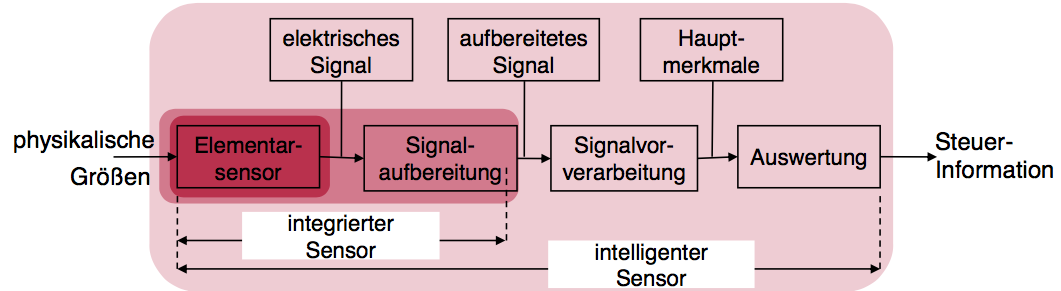
\includegraphics [scale=0.5]{sensor}
\end{figure}

\begin{compactitem}
    \item \textbf{Elementarsensor}: Aufnahme einer Messgröße und Abbildung auf Signal
    \item \textbf{Integrierter Sensor}: zus. Signalaufbereitung (Verstärkung, Filterung, Linearisierung,
    Normierung).
    \item \textbf{Intelligenter Sensor}: integrierter Sensor mit rechnergesteuerter Auswertung
\end{compactitem}

\subsection{Klassifizierung von Sensoren}
\begin{compactitem}
    \item \textbf{Interne Sensoren}: Erfasst innere Zustände. Bestimmung von Lage und Position durch
    Neigung, Orientierung, Drehrichtung, Beschleunigung und Lenkwinkel. \\
    \begin{inparaitem}
        \item Positionssensor
        \item Geschwindigkeitssensor
        \item Beschleunigungssensor
        \item Inertial Navigation System
    \end{inparaitem}
    \item \textbf{Externe Sensoren}: Information aus Umwelt über dessen Zustand. Bestimmung von Position
    und Orientierung in Bezug auf Umwelt, Beschaffenheit der Umwelt, Kommandos.
    \begin{compactitem}
        \item \textbf{Aktive Sensoren}: Simulation der Umwelt durch Eintrag der Energie, Messen und
        Auswerten der Antwort.\\
        \begin{inparaitem}
            \item Ultraschall
            \item Infrarot
            \item Laser-Entfernungsmesser
            \item Lichtschnittverfahren
        \end{inparaitem}
        \item \textbf{Passive Sensoren}: Umwelt vorhandene Signale werden gemessen und ausgewerten.\\
        \begin{inparaitem}
            \item Tastsensoren
            \item Photodetektoren
            \item Kameras
            \item Mikrophone
        \end{inparaitem}
    \end{compactitem}
\end{compactitem}
